\documentclass[UTF8]{ctexart}
\CTEXsetup[format={\Large\bfseries}]{section}

\usepackage[a4paper, left = 2cm, right = 2cm]{geometry}
\usepackage{titlesec}
\usepackage{enumerate}
\usepackage{graphicx}
\usepackage{float} 
\usepackage{subfigure}
\usepackage{fancyhdr}
\usepackage{amsmath}
\usepackage{tikz}
\usepackage{fancyhdr}
\usepackage{makecell}
\usepackage{ccaption}
\usepackage[justification=centering]{caption}
\usepackage{multirow}
\usepackage{amsfonts}
\usepackage{amssymb}
\usepackage{booktabs}
\usepackage{siunitx}
\usepackage{setspace}
\usepackage{diagbox}


\usetikzlibrary{snakes}

\pagestyle{fancy}
\fancypagestyle{normal}{%
  \fancyhead{} % clear all header fields
  \fancyhead[L]{\leftmark}}
\fancypagestyle{special}{%
  \fancyhead{} % clear all header fields
  \fancyhead[L]{\rightmark}}



\setlength{\headheight}{13.6pt}

\title
{Part I\quad Experimental Design and Analysis
\\{\large Based on lectures by Shibing Li}
\\{\normalsize Notes taken by Wei Xiong}
\\{\normalsize Qiqiao Festival 2021}
}
\date{}
\pagestyle{fancyplain} %使用fancyplain风格
\fancyhf{} %清除所有页眉页脚

\begin{document}
\maketitle

{\normalsize These notes are not endorsed by the lecturers, and I have modified them (often
significantly) after lectures. They are nowhere near accurate representations of what
was actually lectured, and in particular, all errors are almost surely mine.}	

\newpage %\chapter{CHAPTER 1. Homework Solution}去掉了

\setcounter{page}{1}

\pagestyle{fancy}

\lhead{Les 1 \quad 绪论}		 %设置页眉左侧
\chead{}			%设置页眉中间
\rhead{试验设计与数据处理}			%设置页眉右侧为leftmark
\lfoot{}			%设置页脚左侧为rightmark
\cfoot{\thepage}			%设置页脚中间为页码
\rfoot{}			%设置页脚右侧为"右边页脚"
\clearpage   



\section{试验设计与数据分析 · 绪论}
\subsection{看似“无用”的前言}
\begin{center}
播下一种态度,收获一种行动;\\
播下一种行动,收获一种习惯;\\
播下一种习惯,收获一种性格;\\
播下一种性格,收获一种命运。
\end{center}

\emph{
\begin{enumerate}[•]
\item 态度指的是一种正在进行时的一种状态,行动是状态的积分,最小单元为一个番茄钟。
\item 习惯是是行动的宏观表述,但完成事件不仅仅需要一种行动,更多的是对过去时的一种概述。
\item 性格是习惯所得资源以及现有知识储备的一种选择,思考一下自己想拥有一个怎样的性格(这样的性格需要什么物质来支撑)。
\item 命运这东西——尽人事,听天命。
\end{enumerate}
}

\begin{center}
\item 春蚕到死丝方尽,蜡炬成灰泪始干
\end{center}

\begin{center}
\item 无知→谦虚→包容
\end{center}

\emph{学如逆水行舟,不进则退。故谦虚并非指沉寂,更多的是一种谦和。}
\par \emph{——正所谓“谦和以为本,进取方为道”。}

\subsection{试验设计与数据分析的引入}
\textbf{Example.}
  锂离子二次电池分别应用于锂离子电池、电动自行车、手机、笔记本电脑时,需要关注什么参数?这些参数如何建立模型研究?又怎样实现模型到实体的转换?\\
\par 我们用四个步骤来解决这个问题:
\begin{enumerate}[(i)]
\item 材料制备:按照工艺流程图所需材料和设备环境进行操作
\item 电极制作:按照相应的工艺流程图进行组装
\item 电池组装:在相应环境,按照电池结构示意图进行进一步组装
\item 性能测试:将电化学分析设备所得数据进行绘图以及进一步处理
\end{enumerate}


\subsection{实验与试验的区别}
\begin{center}
\item 实验:已知某个结论去验证,已知方法的操作(验证性)
\item 试验:未知某个结论去探索,未知方法的探索(探索性)
\end{center}

\begin{enumerate}[•]
\item 实验:根据所获得的知识能够证实或证伪的,带有强烈的目的性;
\item 试验:结果是根据现有的知识不能证实和证伪的,经验积累。
\item 实验:属于重复前人的东西,对理论进行的实践;
\item 试验:探索未知领域,由实践归纳理论。
\item 实验:把理论知识用于实际体系;
\item 试验:是给不确定的东西找结论。
\end{enumerate}

\begin{spacing}{1.5}
\par \emph{“不要看不起实验,更不要低估试验。}
\par \emph{重复实验的难点即为“纸上得来终觉浅,绝知此事要躬行”:其一是信息的传递损耗,其二是参数的控制。至于试验,是在实验的基础之上,加上一些科学性的研究方法。}
\par \emph{所以,连实验都做不好,又怎能寄希望于试验成功?”}
\end{spacing}

\subsection{试验设计与数据处理的定义}

\begin{enumerate}[•]
\item 试验设计:以概率论与数理统计学为理论基础,为获得可靠试验结果和有用信息,科学安排试验的一种方法论,亦是研究如何高效而经济地获取所需要的数据与信息的方法。
\begin{itemize}
\item 是对一个过程或系统的输入变量作一些有目的的改变,以使能够观察到和识别出引起输出相应变化的缘由。
\end{itemize}
\item 数据处理:对试验测量结果或观察数据进行分析计算,从而得出可靠且规律性的结果。
\end{enumerate}

\subsection{为什么要进行试验设计}

\begin{enumerate}[•]
 \item 试验设计被广泛应用于农业领域、道路交通、桥梁、工业产品领域。以工业试验为例,其可以:升级产品功能、提高产品质量、延长产品寿命、降低能源消耗等等。
\begin{itemize}
\item 好的试验方案:减少试验次数、缩短试验周期、降低试验费用、得到正确的结论、有较好的试验结果。
\item 试验方案不当:增加试验次数、延长试验周期、造成人力、时间浪费、不仅难以达到预期效果,甚至造成试验的全盘失败。
\end{itemize}
\end{enumerate}

\subsection{如何进行试验设计}
\textbf{Example.}
某五金厂生产某种牌号的弹簧。为提高弹性、防止弹簧的断裂,进行热处理回火工艺试验。根据专业知识和生产经验,选取回火温度、保温时间和工件重量三个因素,每个因素取三个水平进行试验。希望通过试验确定最好的生产条件。

\begin{center}
\begin{tabular}{cccc}
\hline
\diagbox{水平}{因素} & 回火温度A & 保温时间B & 工件质量C  \\
\hline
1 & 440   & 3min  & 7.5公斤 \\
2 & 470   & 4min  & 9.0kg  \\
3 & 500   & 5min  & 10.5kg \\
\hline
\end{tabular}
\end{center}



\subsubsection{单因素轮换法}
\begin{enumerate}[•]
\item 固定A为$A_1$、B为$B_1$,改变C的水平,即做3次实验$A_1$$B_1$$C_1$、$A_1$$B_1$$C_2$、$A_1$$B_1$$C_3$。$A_1$$B_1$\textbf{$C_2$}最好
\item 固定A为$A_1$、C为$C_2$,改变B的水平,即做3次实验$A_1$$C_2$$B_1$、$A_1$$C_2$$B_2$、$A_1$$C_2$$B_3$。$A_1$$C_2$\textbf{$B_2$}最好
\item 固定B为$B_2$、C为$C_2$,改变A的水平,即做3次实验$B_2$$C_2$$A_1$、$B_2$$C_2$$A_2$、$B_2$$C_2$$A_3$。$B_2$$C_2$\textbf{$A_1$}最好
\end{enumerate}
\par 故最佳工艺为$A_1$$B_2$$C_2$

\subsubsection{全因子试验}
\begin{center}
\begin{tabular}{cccccc}
\hline
试验编号 & 试验条件 & 试验编号 & 试验条件 & 试验编号 & 试验条件  \\
\hline
1 & $A_1$$B_1$$C_1$ & 10 & $A_2$$B_1$$C_1$ & 19 & $A_3$$B_1$$C_1$ \\
2 & $A_1$$B_1$$C_2$ & 11 & $A_2$$B_1$$C_2$ & 20 & $A_3$$B_1$$C_2$ \\
3 & $A_1$$B_1$$C_3$ & 12 & $A_2$$B_1$$C_3$ & 21 & $A_3$$B_1$$C_3$ \\
4 & $A_1$$B_2$$C_1$ & 13 & $A_2$$B_2$$C_1$ & 22 & $A_3$$B_2$$C_1$ \\
5 & $A_1$$B_2$$C_2$ & 14 & $A_2$$B_2$$C_2$ & 23 & $A_3$$B_2$$C_2$ \\
6 & $A_1$$B_2$$C_3$ & 15 & $A_2$$B_2$$C_3$ & 24 & $A_3$$B_2$$C_3$ \\
7 & $A_1$$B_3$$C_1$ & 16 & $A_2$$B_3$$C_1$ & 25 & $A_3$$B_3$$C_1$ \\
8 & $A_1$$B_3$$C_2$ & 17 & $A_2$$B_3$$C_2$ & 26 & $A_3$$B_3$$C_2$ \\
9 & $A_1$$B_3$$C_3$ & 18 & $A_2$$B_3$$C_3$ & 27 & $A_3$$B_3$$C_3$ \\
\hline
\end{tabular}
\end{center}

\subsubsection{正交试验设计}
\begin{center}
\begin{tabular}{ccccc}
\hline
试验编号 & 因素A & 因素B & 因素C & 试验条件  \\
\hline
1 & 1 & 1 & 1 & $A_1$$B_1$$C_1$ \\
2 & 1 & 2 & 2 & $A_1$$B_2$$C_2$ \\
3 & 1 & 3 & 3 & $A_1$$B_3$$C_3$ \\
4 & 2 & 1 & 2 & $A_2$$B_1$$C_2$ \\
5 & 2 & 2 & 3 & $A_2$$B_2$$C_3$ \\
6 & 2 & 3 & 1 & $A_2$$B_3$$C_1$ \\
7 & 3 & 1 & 3 & $A_3$$B_1$$C_3$ \\
8 & 3 & 2 & 1 & $A_3$$B_2$$C_1$ \\
9 & 3 & 3 & 2 & $A_3$$B_3$$C_2$ \\
\hline
\end{tabular}
\end{center}

\subsubsection{均匀试验设计}
\begin{center}
\begin{tabular}{ccccc}
\hline
试验编号 & 因素A & 因素B & 因素C & 试验条件  \\
\hline
1 & 1 & 3 & 2 & $A_1$$B_3$$C_2$ \\
2 & 2 & 1 & 3 & $A_2$$B_1$$C_3$ \\
3 & 3 & 2 & 1 & $A_3$$B_2$$C_1$ \\
\hline
\end{tabular}
\end{center}

\subsubsection{小结}
\begin{enumerate}[•]
\item 单因素轮换法
\begin{itemize}
\item 一般能取得一定效果。
\item 局限性大,很难做到最优。
\item 一些好的组合没有被试验发现,如$A_1$$B_2$$C_3$。
\item 各因素考察不均匀。
\begin{center}
\begin{tabular}{cccccccccc}
\toprule
因素水平&$A_1$&$A_2$&$A_3$&$B_1$&$B_2$&$B_3$&$C_1$&$C_2$&$C_3$\\ 
\midrule
试验次数& 7&1  &1  &4  &4  &1  &1  &7  &1  \\
\bottomrule
\end{tabular}
\end{center}

\end{itemize}
\item 全因子试验
\begin{itemize}
\item 全面,能选出最佳的方案。
\item 因素水平较多时,试验次数激增。如对于同样为3因素的试验,水平数为3、4、5、7、10时,试验次数依次为27、64、125、343、1000。
\item 太多的试验次数在实际生产或研究中心是无法实现的。
\end{itemize}
\item 正交试验设计
\begin{itemize}
\item 试验次数明显减少,有更大的实用性。
\item 试验整齐可比,均衡分散。
\item 试验后数据便于后续分析、计算。
\end{itemize}
\item 均匀试验设计
\begin{itemize}
\item 与正交试验设计相比,均匀设计仅考虑试验安排的均匀性,不考察可比性,所以试验次数剧减。
\item 均匀设计对于地因素、低水平的试验没有优势,但对于多因素、多水平的试验可以大大减少试验次数。
\item 例如3因素,9水平的试验,全因子试验需要729次,正交试验需81次,均匀设计仅需9次。
\end{itemize}
\end{enumerate}

\subsection{为什么需要对数据进行处理}
\begin{enumerate}[•]
\item 对试验测量结果或观察数据进行分析计算,从而得出可靠且规律性的结果,依据这个规律性的结果对生产、试验进行预测或控制,进而掌握客观事物的发展规律,使之服从和服务于人类。
\begin{itemize}
\item 分清各个试验因素对试验指标影响的大小顺序,找出主要因素,抓住主要矛盾;
\item 了解因素与试验指标间的规律性,即每个因素的水平改变时,指标是怎么样变化的;
\item 了解各因素之间的相互影响情况,即因素之间的交互作用情况;
\item 迅速找出最优的生产条件或工艺,确定最优方案,并能预测在最优生产条件下的试验指标值;
\item 了解试验误差的大小,从而提高试验的精度;
\item 明确为寻找最优或工艺条件而进一步试验的研究方向。
\end{itemize}
\end{enumerate}

\subsection{如何进行数据处理}
\subsubsection{直观分析法}
\begin{enumerate}[•]
\item 直观分析法:通过对试验结果的简单计算,直接分析比较确定最佳效果。
\par 直观分析法主要可以解决以下两个问题:
\begin{itemize}
\item 确定因素最佳水平。
\par 计算出每个因素每一水平的试验指标值的总和与平均值,通过比较确定最佳水平。
\item 确定影响试验指标的因素主次地位。
\par 解决这一问题采用极差法,某个因素的极差定义为该因素在不同水平下的指标平均值的最大值与最小值之间的差值。
\end{itemize}
\end{enumerate}
\textbf{Example.}
某水泥厂为了提高水泥的强度,需要通过试验选择最好的生产方案,经研究,有3个因素影响水泥的强度,分别为生料中矿化剂用量、烧成强度、保温时间,每个因素都考虑三个水平。具体情况如表,试验的考察指标为28天的抗压强度(MPa),分别为44.1,45.3,46.7,48.2,46.2,47.0,45.3,43.2,46.3,问这3个因素的3个水平如何安排,才能获得最高的水泥抗压强度。
\begin{center}
\begin{tabular}{cccc}
\hline
\diagbox{水平}{因素}& \makecell*[c]{A\\矿化剂用量($\%$)} & \makecell*[c]{B\\烧成温度($^{\circ}$C)} & \makecell*[c]{C\\保温时间(min)} \\
\hline
1 & 2   & 1350  & 20 \\
2 & 4   & 1400  & 30  \\
3 & 6   & 1450  & 40 \\
\hline
\end{tabular}
\end{center}


\begin{center}
\begin{tabular}{ccccc}
\hline
\diagbox{水平}{因素}& \makecell*[c]{A\\矿化剂用量($\%$)} & \makecell*[c]{B\\烧成温度($^{\circ}$C)} & \makecell*[c]{C\\保温时间(min)}& \makecell*[c]{考察指标\\抗压强度(MPa)} \\
\hline
1 & 1   & 1  & 1 & 44.1\\
2 & 1   & 2  & 2 & 45.3\\
3 & 1   & 3  & 3 & 46.7\\
4 & 2   & 1  & 2 & 48.2\\
5 & 2   & 2  & 3 & 46.2\\
6 & 2   & 3  & 1 & 47.0\\
7 & 3   & 1  & 3 & 45.3\\
8 & 3   & 2  & 1 & 43.2\\
9 & 3   & 3  & 2 & 46.3\\
\hline
$K_1$& 136.1   & 137.6  & 134.3 & \\
$K_2$& 141.4   & 134.7  & 139.8 & 各个因素水平指标和 \\
$K_3$& 134.8   & 140.0  & 138.2 &  \\
\hline
$k_1$=$K_1$/3& 45.67   & 45.87  & 44.77 &  \\
$k_2$=$K_2$/3& 47.13   & 44.90  & 46.60 & 各个因素水平指标和平均值\\
$k_3$=$K_3$/3& 44.93   & 46.67  & 46.07 &  \\
\hline
极差& 2.20   & 1.77  & 1.83 & 表中最好方案为  \\
优方案&$A_2$   & $B_3$  & $C_2$ &  第4号试验\\
\hline
\end{tabular}
\end{center}

\subsubsection{方差分析法}
\begin{enumerate}[•]
\item 方差分析法:把实验数据的波动分解为各个因素的波动与误差波动,然后对它们的平均波动进行比较。
\begin{itemize}
\item 将总的偏差平方和(${S_T}^2$)分解为反映必然性的各个因素的偏差平方和(${S_A}^2$,${S_B}^2$…)与反应偶然性的误差平方和(${S_e}^2$),并计算比较它们的平均偏差平方和,以找出对试验数据起决定性影响的因素。
\end{itemize}
\end{enumerate}

\textbf{Example.}
考察生产某化工产品时反应温度A($^{\circ}$C)对收率y($\%$)的影响。为此,比较两个反应温度$A_1$=30$^{\circ}$C,$A_2$=40$^{\circ}$C.这是一个单因素两水平的试验,试验结果如下表:
\begin{center}
\begin{tabular}{ccccccc}
\toprule
\diagbox{水平}{试验号}& 1& 2& 3& 4& 5& 平均值\\
\midrule
$A_1$=30$^{\circ}$C & 75& 78& 60& 61& 83&  $\bar{y_1}$=71.4\\
$A_2$=40$^{\circ}$C & 89& 62& 93& 71& 85&  $\bar{y_2}$=80.0\\
\bottomrule
\end{tabular}
\end{center}

\par 取水平1,平均收率为71.4,可表示水平1各次试验对试验指标的影响。
\par 取水平2,平均收率为80.0,可表示水平2各次试验对试验指标的影响。
\begin{equation}
\bar{y}=\frac{1}{10}(75+78+...+85)=75.7
\end{equation}
\par 全部实验值与总的平均值之差的离差平方和反映\textbf{指标观测值的总波动},记为${S_T}^2$。
\begin{equation}
{S_T}^2=(75-75.7)^2+(78-75.7)^2+...(85-75.7)^2=1294.10
\end{equation}
\par \textbf{试验误差},用误差离差平方和 ${S_e}^2$表示。
\begin{equation}
{S_e}^2=(75-71.4)^2+...+(83-71.4)^2+(89-80.0)^2+...(85-80.0)^2=1109.20
\end{equation}
\par ${S_A}^2$反映了因素的\textbf{水平改变引起的指标波动},其中包含试验误差的影响。
\begin{equation}
{S_A}^2=5(71.4-75.7)^+5(80.0-75.7)^2=184.90
\end{equation}
\par 有了${S_e}^2$和${S_A}^2$,还不能比较出由于因素水平和误差引起的波动,因为离差平方和不仅与数据本身有关,还与数据的个数有关。
\par 为了消除个数的影响,采用平均离差平方和${S_e}^2$/$f_e$和${S_A}^2$/$f_A$进行比较。
\par 对于${S_e}^2$而言,其中的10个数据满足两个关系式:
\begin{equation}
\bar{y_1}=\frac{1}{5}(75+78+...+83)=71.4,\quad \bar{y_2}=\frac{1}{5}(89+62+...+85)=80.0
\end{equation}
\begin{equation}
\therefore f_{e}=10-2=8
\end{equation}
\par 对于${S_A}^2$而言,其中的2个数据有一个关系式
\begin{equation}
\bar{y}=\frac{1}{2}(\bar{y_1}+\bar{y_2})=\frac{71.4+80.0}{2}=75.7
\end{equation}
\begin{equation}
\therefore f_{A}=2-1=1
\end{equation}
\par 对于${S_T}^2$而言,其中的10个数据有一个关系式
\begin{equation}
\bar{y}=\frac{1}{10}(75+78+...+85)=75.7
\end{equation}
\begin{equation}
\therefore f_{T}=10-1=9
\end{equation}
\par $F_{A}$接近于1,表明因素水平改变对试验指标的影响与试验误差对试验指标的影响相当,可以认为\textbf{因素水平之间没有显著差异}。
\par 反之,则可以认为因素水平之间有显著差异或因素对指标影响显著。
\begin{equation}
F_{A}=\frac{{S_A}^{2}/f_{A}}{{S_e}^{2}/f_{e}}=\frac{184.90/1}{1109.20/8}=1.33
\end{equation}
\par 对于a=0.05,查表得
\begin{equation}
F_{0.05}(1,8)=5.32\textgreater1.33
\end{equation}
\par 在此显著性水平下,反应温度A对试验指标影响不显著,说明试验结果波动主要来源于误差
\subsubsection{因素-指标关系趋势图分析方法}
\par 计算各因素各个水平平均试验指标,采用因素的水平作横坐标,各水平的平均试验指标作为纵坐标绘制因素-指标关系趋势图,找出个水平与试验指标间的变化规律。
\par 以1.8.1 直观分析法中表格2为例,用Origin绘制因素-指标关系趋势图:

\begin{figure}[H]
\begin{center}
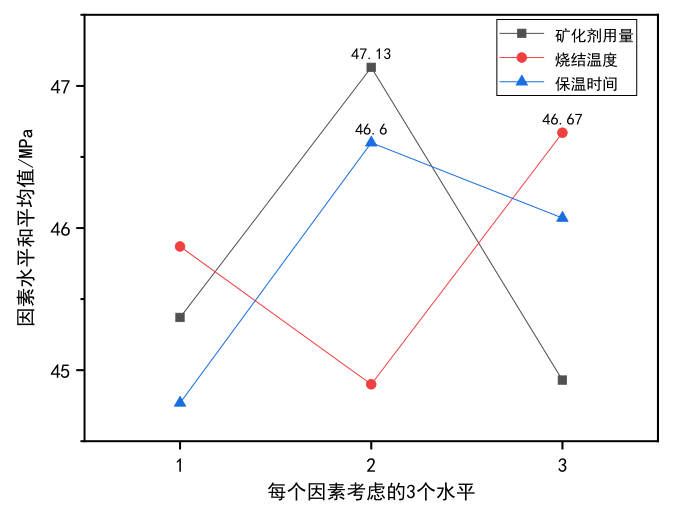
\includegraphics[height=16\baselineskip]{FIG/N1.png}
\captionsetup{font={footnotesize}}
\end{center}
\end{figure}
\par 显然,为了获得优方案应选择$A_2$$B_3$$C_2$。

\setcounter{equation}{0}

\subsubsection{回归分析法}
\par 回归分析法是用来寻找试验因素与试验指标之间是否存在函数关系的一种方法。
\par \textbf{Example.} 为研究某合成物的转化率T与试验中高端压强p(atm)的关系,得到下表数据。用最小二乘法确定转化率与压强的经验公式。

\begin{center}
\begin{tabular}{cccccc}
\toprule
p/atm&2&4&5&8&9\\ 
\midrule
T/$\%$ & 2.01&2.98  &3.50  &5.02  &5.07\\
\bottomrule
\end{tabular}
\end{center}
\par 用Origin对此表数据进行线性拟合:
\begin{figure}[H]
\begin{center}
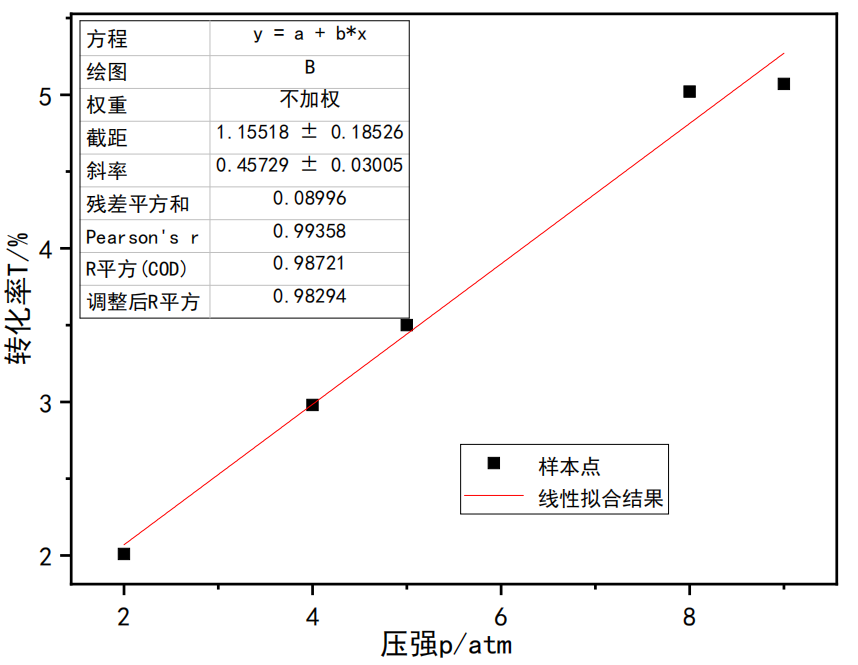
\includegraphics[height=20\baselineskip]{FIG/N2.png}
\captionsetup{font={footnotesize}}
\end{center}
\end{figure}

\begin{equation}
\begin{aligned}\notag 
L_{xy}&=\sum\limits_{i=1}^nx_{i}y_{i}-n\bar{x}\bar{y}=119.23-5\times5.6\times3.716=15.182\\
L_{xx}&={\sum\limits_{i=1}^nx_{i}^{2}-n(\bar{x})^2}=190-5\times5.6^{2}=33.2\\
b&=\frac{L_{xy}}{L_{xx}}=\frac{15.182}{33.2}=0.4573\\
a&=\bar{y}-b\bar{x}=3.716-0.4573\times5.6=1.155\\
\therefore T&=1.155+0.4573\\
\end{aligned}
\end{equation}

\begin{enumerate}[•]
\item 一元线性回归方程:
\begin{equation}
y_{i}=a+bx_{i} 
\end{equation}

\begin{itemize}
\item $a,b:$ 回归系数(regression coefficient)
\item $y_{i}:$ 回归值/拟合值,由$x_{i}$代入回归方程计算出的值
\item $e_{i}:$ 残差,计算值$y_{i}$与试验值$y_{0}$之差
\end{itemize}
\begin{equation}
e_{i}=y_{i}-y_{0} 
\end{equation}
\begin{itemize}
\item $SS_{e}$残差平方和:
\end{itemize}
\begin{equation}
SS_{e}=Q=\sum_{i=1}^ne_{i}^{2}=\sum_{i=1}^n(y_{i}-y_{0})^{2}=\sum_{i=1}^n[(y_{i}-(a+bx_{i})]^2     
\end{equation}
\end{enumerate}
\par 残差平方和最小时,回归方程与试验值的拟合程度最好


\begin{equation}
\left\{
\begin{aligned}
&\frac{\partial Q}{\partial a}=-2\sum_{i=1}^n(y_{i}-a-bx_{i})=0\\
&\frac{\partial Q}{\partial b}=-2\sum_{i=1}^n(y_{i}-a-bx_{i})x_{i}=0
\end{aligned}
\right.
\end{equation}
\par 正规方程组(normal equation):

\begin{equation}
\left\{
\begin{aligned}
&na+b\sum_{i=1}^nx_{i}=\sum_{i=1}^ny_{i}\\
&a\sum_{i=1}^nx_{i}+b\sum_{i=1}^nx_{i}^{2}=\sum_{i=1}^nx_{i}y_{i}
\end{aligned}
\right.
\end{equation}


\par 解正规方程组:

\begin{equation}
a=\bar{y}-b\bar{x}
\end{equation}


\begin{equation}
b=\frac{n\sum\limits_{i=1}^nx_{i}y_{i}-(\sum\limits_{i=1}^nx)(\sum\limits_{i=1}^ny)}
{\sum\limits_{i=1}^nx_{i}^{2}-(\sum\limits_{i=1}^nx_{i})^{2}}
=\frac{\sum\limits_{i=1}^nx_{i}y_{i}-n\bar{x}\bar{y}}{\sum\limits_{i=1}^nx_{i}^{2}-n(\bar{x})^2}
\end{equation}

\par 又有,
\begin{equation}
\left\{
\begin{aligned}
&L_{xy}=\sum\limits_{i=1}^n(x_{i}-\bar{x})(y_{i}-\bar{y})=\sum\limits_{i=1}^nx_{i}y_{i}-n\bar{x}\bar{y}\\
&L_{xx}=\sum\limits_{i=1}^n(x_{i}-\bar{x})^{2}={\sum\limits_{i=1}^nx_{i}^{2}-n(\bar{x})^2}\\
\end{aligned}
\right.
\end{equation}
\par 即,
\begin{equation}
b=\frac{L_{xy}}{L_{xx}}
\end{equation}

\subsection{试验设计与数据处理的发展和应用}
\begin{enumerate}[•]
\item 20世纪后期,提出“信噪比设计”和“产品三次设计”
\begin{itemize}
\item 信噪比设计:信号功率与噪音功率的比值,用来评价仪器和设备质量的好坏。
\item 产品三次设计:系统设计、参数设计、容差设计,使整机的零件各参数合理搭配,保证采用低级价廉的零部件,仍能确保整体质量和高的稳定性。
\end{itemize}
\item 我国试验设计方法发展
\begin{itemize}
\item 1948年,范福仁, 《田间试验之统计与分析》。
\item 1970年,华罗庚推广优选法、统筹法。
\item 1978年,优选法用于五粮液获得成功。
\item 1978年,方开泰、王元创造均匀设计法。
\end{itemize}
\end{enumerate}

\subsection{本章教学大纲}
\begin{enumerate}[•]
\item 掌握
\begin{itemize}
\item 试验设计的基本原理和方法,能够利用相关原理设计材料研究中的研究方案,同时可以对试验结果进行科学的分析。
\item Excel软件进行作图和数据处理以及Origin进行数据作图。
\end{itemize}
\item 考察
\begin{itemize}
\item 试验设计与数据分析的基本概念、基本步骤、简单应用。
\end{itemize}
\item 使用教材与推荐参考书目
\begin{itemize}
\item 李云雁,胡传荣.《试验设计与数据处理》化学工业出版社,2008
\item 郑少华等.《试验设计与数据处理》中国建材工业出版社,2004
\item 邱轶兵.《试验设计与数据处理》中国科学技术大学出版社,2008
\item 赵选民.《试验设计方法》科学出版社,2006
\item 刘文卿.《实验设计》清华大学出版社,2005
\item 田胜元等.《实验设计与数据处理》建筑工业出版社,1988
\end{itemize}
\end{enumerate}

\newpage
\setcounter{equation}{0}

\lhead{Les 2 \quad 试验数据的误差分析}		 %设置页眉左侧
\chead{}			%设置页眉中间
\rhead{试验设计与数据处理}			%设置页眉右侧为leftmark
\lfoot{}			%设置页脚左侧为rightmark
\cfoot{\thepage}			%设置页脚中间为页码
\rfoot{}			%设置页脚右侧为"右边页脚"
\clearpage   


\section{试验设计的误差分析}
\subsection{真值与平均值}
\subsubsection{真值}
\par 真值(true value):在某一时刻和某一状态下,某量的客观值或实际值。

\subsubsection{算术平均值}
\begin{equation}
\bar{y}=\frac{{y_1}+{y_2}+...+{y_n}}{n}
\end{equation}


\begin{enumerate}[•]
\item 算术平均值只适用于有限个数值。
\item 同样试验条件下,如果多次试验值服从正态分布,则算数平均值是这组数据中的最佳值或最可信赖值。

\par 正态分布——概率密度函数
\begin{equation}
f(x)=\frac{1}{\sqrt{2\pi}\sigma}\exp[-\frac{(x-\mu)^2}{2\sigma^2}],\ x\in \mathbb{R} 
\end{equation}

\begin{itemize}
\item 典型正态分布:测量误差;炮弹落点分布;人的身高、体重;化工产品中某成分的含量;农作物的收获量。
\end{itemize}
\item 正态分布的特点
\begin{itemize}
\item 曲线关于$x=\mu$对称。$\mu$决定曲线的中心位置,称为位置参数。
\item 为单峰曲线,在$x=\mu$处有极大值。
\item 曲线有两个拐点,位于$x=\mu+\sigma$处。$\sigma$决定曲线的形状,称为形状参数。
\item 当$\lim\limits_{x\to\infty}$,曲线以x轴为渐近线。
\item 曲线与x轴所围面积为1,代表各种样本值出现概率的总和。
\end{itemize}
\end{enumerate}

\textbf{Proof.}

\begin{equation}
 \begin{aligned}\notag
    f(x)=&\frac{1}{\sqrt{2\pi}\sigma}\exp[-\frac{(x-\mu)^2}{2\sigma^2}]
  \\f(x)'=&\frac{1}{\sqrt{2\pi}\sigma}\times[-\frac{(x-\mu)}{\sigma^2}]\exp[-\frac{(x-\mu)^2}{2\sigma^2}]
  \\f(x)''=&\frac{1}{\sqrt{2\pi}\sigma}\times{[\frac{(x-\mu)}{\sigma^2}]^2}\exp[-\frac{(x-\mu)^2}{2\sigma^2}]
            +\frac{1}{\sqrt{2\pi}\sigma}\times\exp[-\frac{(x-\mu)^2}{2\sigma^2}]\times \frac{-1}{\sigma ^2}
  \\=&\frac{1}{\sqrt{2\pi}\sigma}\times\exp[-\frac{(x-\mu)^2}{2\sigma^2}]\times[\frac{(x-\mu )^2}{\sigma ^4}
            +\frac{-1}{\sigma ^2}]=0
 \end{aligned}
\end{equation}

\begin{equation}
  \begin{aligned}\notag
    &\therefore[\frac{(x-\mu )^2}{\sigma ^4}+\frac{-1}{\sigma ^2}]=0
    \\&\therefore x=\mu \pm \sigma 
  \end{aligned}
\end{equation}

\subsubsection{加权平均值}
\begin{equation}
  \bar{x_\omega }=\frac{\omega_{1}x_{1}+\omega_{2}x_{2}+\cdots +\omega_{n}x_{n}}{\omega_{1}+\omega_{2}+\cdots +\omega_{n}}
                 =\frac{\sum\limits_{i=1}^n\omega_{i}x_{i}}{\sum\limits_{i=1}^n\omega_{i}}
\end{equation}
  
\begin{enumerate}[•]
  \item 不同的方法获得的,或由不同的试验人员得到的,采用加权平均值。
    \begin{itemize}
      \item 例:GPA计算
    \end{itemize} 
  \item 在每一个数相同的情况下,加权平均值就等于算数平均值。
\end{enumerate}

\subsubsection{对数平均值}
\par 设两个数:\ $x_{1}\textgreater0,\  x_{2}\textgreater0$,\ 则
\begin{equation}
\bar{x_L}=\frac{x_{1}-x_2}{\ln {x_1}-\ln {x_2}}=\frac{x_{1}-x_2}{\ln \frac{x_1}{x_2}}=\frac{x_{2}-x_1}{\ln \frac{x_2}{x_1}}
\end{equation}
\begin{enumerate}[•]
  \item 若数据的分布具有对数特性,则宜使用对数平均值
  \item 对数平均值$\leqslant $算术平均值
  \item 如果$\frac{1}{2}\leqslant \frac{x_1}{x_2} \leqslant 2 $时,可用算术平均值代替。
\end{enumerate}

\subsubsection{调和平均值}
  \par 设有n个正试验值:$x_{1},x_{2},\ldots ,x_{n}$,则:
  \begin{equation}
  \frac{1}{H}=\frac{\frac{1}{x_1}+\frac{1}{x_2}+\ldots +\frac{1}{x_n}}{n}=\frac{\sum\limits_{i=1}^n\frac{1}{x_i}}{n}
  \end{equation}
  \begin{enumerate}[•]
    \item 其给予较小值更高的权重,常用在涉及到一些量的倒数有关的场合
     \begin{itemize}
      \item 例:计算是否偏科
    \end{itemize} 
    \item 调和平均值$\leqslant$几何平均值$\leqslant$算术平均值
  \end{enumerate}

\setcounter{equation}{0}
\subsection{误差的基本概念}
\subsubsection{误差公理}
\par \textbf{Axiom.} 测量结果都有误差,误差自始至终存在于一切科学试验和测量过程中。
\par  例:用台式血压计测量人体血压\\
 测量仪器、测量方法、测量人员、测量环境、测量对象等都会产生误差。

 
\subsubsection{绝对误差}
\par 定义:被测量的测量值与其真值之差。

\begin{equation}
  \Delta x=x-x_{t}
\end{equation}
\begin{equation}
    x_{t}\approx x\pm \left\lvert \Delta x\right\rvert _{max}
\end{equation}


\begin{enumerate}[•]
\item $\Delta x$为绝对误差;$x$为测得值;$x_t$为被测量的真值。
  \begin{itemize}
  \item 真值一般是未知的,通常用最大的绝对误差来估计其大小范围。
  \item 最大绝对误差的估算:用仪器的精密等级;用仪器的最小刻度
  \end{itemize} 
\item 关于绝对误差
\begin{itemize}
\item 一般说的误差就是绝对误差。
\item 绝对误差具有确定的大小、计量单位和正负号。
      反映测量值偏离真值的大小与方向,通常用于同一量级的同种量的测量结果的误差比较。
\item 绝对误差数值大小与所取单位有关。

\end{itemize} 
\end{enumerate}

\textbf{Example.}
某加工车间加工一批直径为50mm的轴,抽检两根轴的直径分别为49.9mm和49.8mm,两根轴的绝对误差为:
\begin{equation}\notag
  \Delta x_{1}=49.9-50=-0.1mm
\end{equation}
\begin{equation}\notag
  \Delta x_{2}=49.8-50=-0.2mm
\end{equation}

\subsubsection{相对误差}
\begin{equation}
  r=\frac{\delta  x}{x_{t}}\approx \frac{\delta x}{x}
\end{equation}



\begin{enumerate}[•]
\item 关于相对误差
  \begin{itemize}
  \item 相对误差是一个比值,其数值与所取单位无关,因而是一个无量纲数,通常用百分数表示
  \item 对于相同的被测量,绝对误差可以评定其测量精度的高低,对于不同被测量以及不同的物理量,采用相对误差来评定较为确切。
  \item 绝对误差和相对误差通常适用于单值点测量误差的表示。
  \end{itemize} 
\end{enumerate}

\textbf{Example.}
用电压表分别对A、B两电压表进行测量,试比较两电压测量结果准确度的高低,其测量结果如下:
\begin{equation}\notag
  \begin{aligned}
&x_{A}=100.0V \quad \delta_{A}=1.0V\\
&x_{B}=5.0V \qquad \delta_{B}=0.2V
  \end{aligned}
\end{equation}


\par A、B两电压测量结果的相对误差分别为:
\begin{equation}\notag
  \begin{aligned}
&r_{A}=\frac{\delta_{A}}{x_{A}}=\frac{1.0}{100.0}=1\%\\
&r_{B}=\frac{\delta_{B}}{x_{B}}=\frac{0.2}{5.0}=4\%\\
  \end{aligned}
\end{equation}
\par 通过比较可知A的准确度高于B的准确度。


\subsubsection{算术平均误差}
设试验值$x_i$与算术平均值$\bar{x}$之间的偏差为$d_{i}$,则算术平均误差定义式为:
\begin{equation}
  \Delta =\frac{\sum\limits_{i=1}^n\left\lvert x_{i}-\bar{x}\right\rvert }{n}=\frac{\sum\limits_{i=1}^n\left\lvert d_{i}\right\rvert }{n}
\end{equation}
\begin{enumerate}[•]
\item 关于算术平均误差
  \begin{itemize}
  \item 可能为负,所以一定要取绝对值。
  \item 无法表达出各试验值之间的彼此符合程度。
  \end{itemize} 
\end{enumerate}

\subsubsection{标准误差}
\par 也称作均方根误差、标准偏差,简称为标准差。当实验次数n无限大时,称为总体标准差。
  \begin{equation}
  \sigma =\sqrt{\frac{\sum\limits_{i=1}^n{d{_i}^2}}{n} } 
         =\sqrt{\frac{\sum\limits_{i=1}^n{({x_i}-\bar{x}})^2}{n} } 
         =\sqrt{\frac{\sum\limits_{i=1}^n{x{_i}^2}-\frac{(\sum\limits_{i=1}^n{x{_i})^2}}{n}}{n} } 
  \end{equation}
\par 次数有限称为样本标准差
  \begin{equation}
        s=\sqrt{\frac{\sum\limits_{i=1}^n{d{_i}^2}}{n-1} } 
         =\sqrt{\frac{\sum\limits_{i=1}^n{({x_i}-\bar{x}})^2}{n-1} } 
         =\sqrt{\frac{\sum\limits_{i=1}^n{x{_i}^2}-\frac{(\sum\limits_{i=1}^n{x{_i})^2}}{n}}{n-1} } 
  \end{equation}
\par 表示试验值的精密度,标准差越小,试验数据的精密度越高

\subsection{试验数据误差的来源及分类}
\subsubsection{随机误差}
\begin{enumerate}[•]
\item 关于随机误差
  \begin{itemize}
  \item 定义:以不可预知的规律变化着的误差,绝对误差时正时负,时大时小
  \item 产生的原因:偶然因素
  \end{itemize} 
\item 随机误差的正态统计规律
  \begin{itemize}
  \item 小误差比大误差出现机会多
  \item 正、负误差出现的次数近似相等
  \item 当试验次数足够多时,误差的平均值趋向于0
  \item 可以通过增加试验次数减少随机误差
  \item 随机误差不可完全避免
  \end{itemize} 
\end{enumerate}

\subsubsection{系统误差}
\begin{enumerate}[•]
  \item 关于系统误差
    \begin{itemize}
    \item 定义:一定的试验条件下,由某个或某些因素按照一定的规律起作用而形成的误差
    \item 产生的原因:多方面
    \end{itemize} 
  \item 系统误差的特点
    \begin{itemize}
    \item 系统误差的大小及符号在同一试验中是恒定的
    \item 他不能通过多次试验被发现,也不能通过取多次试验值的平均值的而减小
    \item 只有对系统误差产生的原因有了充分的认识,才能对它进行校正,或设法消除
    \end{itemize} 
  \end{enumerate}

\subsubsection{过失误差}
\begin{enumerate}[•]
  \item 关于过失误差
    \begin{itemize}
    \item 定义:一种显然与事实不符的误差
    \item 产生的原因:试验人员粗心大意造成
    \end{itemize} 
  \item 过失误差的特点
    \begin{itemize}
    \item 可以完全避免
    \item 没有一定的规律
   \end{itemize} 
\end{enumerate}

\subsubsection{三类误差的关系}
\begin{figure}[H]
  \begin{center}
  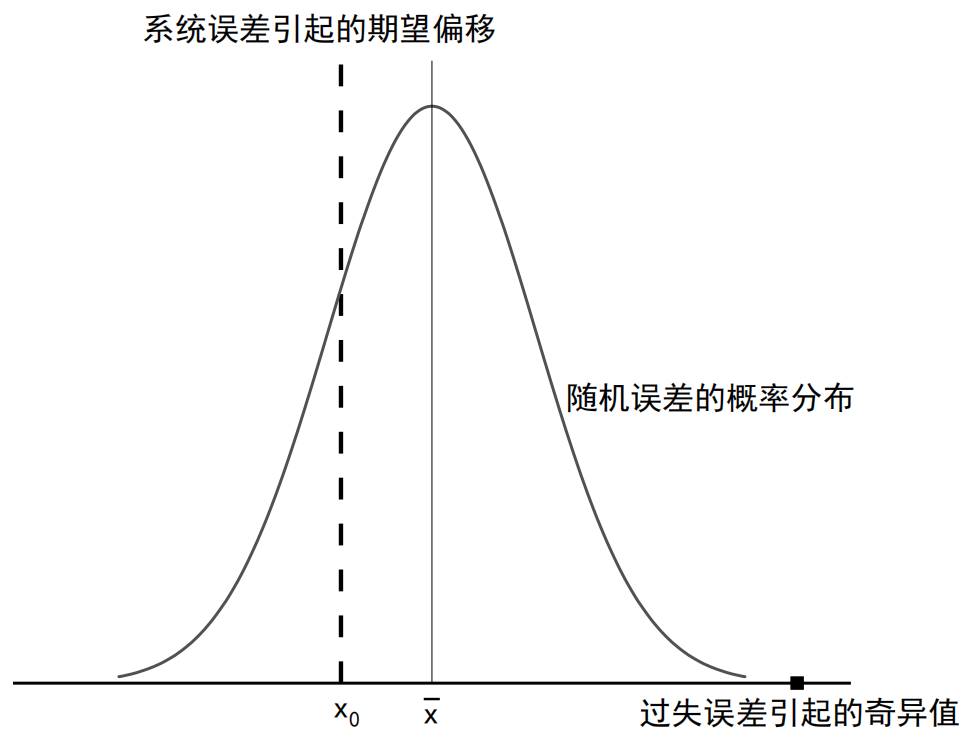
\includegraphics[height=20\baselineskip]{FIG/N3.png}
  \captionsetup{font={footnotesize}}
  \end{center}
  \end{figure}


\subsection{试验数据的精准度}
\subsubsection{精密度}
\begin{enumerate}[•]
  \item 关于精密度
    \begin{itemize}
    \item 反映了随机大小的程度
    \item 在一定的试验条件下,多次试验值的彼此符合程度
    \end{itemize} 
  \item 过失误差的特点
    \begin{itemize}
    \item 可以通过增加试验次数而达到提高数据精密度的目的
    \item 试验数据的精密度是建立在数据用途基础之上的
    \item 试验过程足够紧密,则只需少量几次试验就能满足要求
   \end{itemize} 
  \item 精密度的判断
   \begin{itemize}
    \item 极差:极差越小,精密度越大
    \item 标准差:标准差越小,精密度越大
    \item 方差:方差越小,精密度越大
   \end{itemize} 
\end{enumerate}

\subsubsection{正确度}
\begin{enumerate}[•]
  \item 关于正确度
    \begin{itemize}
    \item 反映系统误差的大小
    \end{itemize} 
  \item 正确度与精密度的关系
    \begin{itemize}
    \item 精密度高并不意味着正确度也高
    \item 精密度不好,但试验次数相当多时,有时也会得到好的正确度
   \end{itemize} 
\end{enumerate}

\subsubsection{准确度}
\begin{enumerate}[•]
  \item 关于准确度
    \begin{itemize}
    \item 反映了系统误差和随机误差的总和
    \item 表示了试验结果与真值的一致程度
    \end{itemize} 
  \item 准确度、正确度、精密度三者关系
    \begin{itemize}
    \item 无系统误差的试验:准确度=精密度+正确度
    \item 有系统误差的试验:极限平均值与真值重合准确度不一定高
   \end{itemize} 
\end{enumerate}

\subsection{随机误差的检验}
\subsubsection{$\chi^2$ 检验}
\begin{enumerate}[•]
\item  目的:在试验数据的总体方差$\sigma ^2$已知的情况下,对试验数据的随机误差或精密度进行检验。
\item 检验步骤:
  \begin{enumerate}[1.]
  \item 计算统计量 $\chi^2$
  \par 若试验数据$x_1$,$x_2$,$\cdots $,$x_n$ 服从正态分布,则
     \begin{equation}\notag
     \chi^{2}=\frac{(n-1)s^2}{\sigma ^2}
     \end{equation}
  \par 服从自由度为$df=n-1$的$\chi^2$分布
  \item 查临界值$\chi^{2}_{\alpha}(df)$
  \par $\alpha$显著性水平一般取0.01或0.05,表示有显著差异的概率
  \item 检验
    \begin{itemize}
    \item 双侧检验
      \begin{equation}\notag
      \chi^{2}_{1-\frac{\alpha}{2}}\textless\chi^{2}\textless\chi^{2}_{\frac{\alpha}{2}}
      \end{equation}
      \par \quad 则判断两方差无显著差异,否则有显著差异
    \item 单侧检验
      \begin{equation}\notag
      \chi^{2}\textgreater\chi^{2}_{1-\alpha}(df)
      \end{equation}
      \par \quad 则判断该方差与原总体方差无显著减小,否则有显著减小(左侧检验)
      \begin{equation}\notag
      \chi^{2}\textless\chi^{2}_{\alpha}(df)
      \end{equation}
      \par \quad 则判断该方差与原总体方差无显著增大,否则有显著增大(右侧检验)
    \end{itemize} 
  \end{enumerate}
\end{enumerate}

\textbf{Example.}
用某分光光度计测定某样品中$Al^{3+}$的浓度,在正常情况下的测定方差为$\sigma^2$=$0.15^2$。
分光光度计检修后,用它测定同样的样品,
测得$Al^{3+}$的浓度(mg/ml)分别为0.142,0.156,0.161,0.145,0.176,0.159,0.165。
试问仪器经过检修后稳定性是否有了显著变化。($\alpha $=0.05)
\begin{equation}\notag
  S^{2}=\frac{\sum\limits_{i=1}^n(x_{i}-\bar{x})^2}{n-1}=0.000135
\end{equation}
\begin{equation}\notag
 \chi^{2}=\frac{(n-1)S^{2}}{\sigma^2}=\frac{(7-1)\times 0.000135}{0.15^2}=0.036
\end{equation}
\par $n=7$,$df=6$,$a=0.05$,查得值$\chi^{2}_{0.975}(6)=1.237$,$\chi^{2}_{0.025}(6)=14.449$
\par $\chi^{2}$落在区间之外,所以仪器经检修后稳定性有显著变化。

\subsubsection{F检验}
\begin{enumerate}[•]
  \item 目的:对两组具有正态分布的试验数据之间的精密度进行比较
  \item 检验步骤:
  \begin{enumerate}[1.]
    \item 计算统计量:
  \par 设有两组试验数据:$x_{1}^{1}$,$x_{2}^{1}$,$\cdots $,$x_{n}^{1}$和$x_{1}^{2}$,$x_{2}^{2}$,$\cdots $,$x_{n}^{2}$都服从正态分布,样本方差分别为$s_{1}^{2}$和$s_{2}^{2}$,则
\begin{equation}\notag
F=\frac{s_{1}^{2}}{s_{2}^{2}}
\end{equation}
\par 服从F分布,第一自由度为$df_{1}=n_{1}-1$,第二自由度为$df_{2}=n_{2}-1$
    \item 查临界值$F^{2}_{\alpha}$($df_{1}$,$df_{2}$)
    \item 检验
    \begin{itemize}
    \item 双侧检验
      \begin{equation}\notag
      F_{1-\frac{\alpha}{2}}(df_{1},df_{2})\textless F \textless F_{\frac{\alpha}{2}}(df_{1},df_{2})
      \end{equation}
      \par \quad 则判断两方差无显著差异,否则有显著差异
    \item 单侧检验
      \begin{equation}\notag
      F\textgreater F_{1-\alpha}(df_{1},df_{2})
      \end{equation}
      \par \quad 则判断方差1比方差2无显著减小,否则有显著减小(左侧检验)
      \begin{equation}\notag
      F\textless F_{\alpha}(df_{1},df_{2})
      \end{equation}
      \par \quad 则判断方差1比方差2无显著减大,否则有显著减大(右侧检验)
    \end{itemize} 
  \end{enumerate}
\end{enumerate}

\textbf{Example.}
用原子吸收光谱法(新法)和EDTA(旧法)测定某废水中$Al^{3+}$的含量($\%$),测定结果如下:
\par 新法:0.163,0.175,0.159,0.168,0.169,0.161,0.166,0.179,0.174,0.173
\par 旧法:0.153,0.181,0.165,0.155,0.156,0.161,0.176,0.174,0.164,0.183,0.179
\begin{enumerate}[(1)]
\item 两种方法是否有显著差异;
\item 新法是否比旧法的精密度有显著提高。($\alpha$=0.05)
\end{enumerate}
\begin{center}
\begin{tabular}{ccccccccccccc}
\toprule
新法&0.163&0.175&0.159&0.168&0.169&0.161&0.166&0.179&0.174&0.173& &VAR(A1:J1) \\ 
\midrule
旧法& 0.153&0.181 &0.165  &0.155  &0.156  &0.161  &0.176  &0.174  &0.164  &0.183 &0.179& VAR(A2:K2)\\
\bottomrule
\end{tabular}
\end{center}
\par 由Excel易得
\begin{equation}\notag
  \begin{aligned}
&S_{1}^{2}=VAR(A1:J1)=4.29\times10^{-5}\quad df_{1}=n_{1}-1=9\\
&S_{2}^{2}=VAR(A2:K2)=1.23\times10^{-4}\quad df_{2}=n_{2}-1=10\\
&F=\frac{S_{1}^{2}}{S_{2}^{2}}=0.350
  \end{aligned}
\end{equation}
\begin{enumerate}[•]
\item 双侧检验:$F_{0.975}(9,10)=0.252$,$F_{0.025}(9,10)=3.779$,F在区间内,没有显著性差异
\item 左侧检验:$F_{0.95}(9,10)=0.319$,$F\textgreater F_{0.95}(9,10)$,故精密度无显著提高
\end{enumerate}

\textbf{Remark.}
\begin{itemize}
\item 双侧检验:$H_{0}:\beta_{1}=k, H_{1}:\beta_{1}\neq k$.
\item 单侧检验:$H_{0}:\beta_{1}\leqslant k, H_{1}:\beta_{1}\geqslant  k$
\item 样本(n-1)和总体(n)的区别:Bessel's correction
\end{itemize} 




\subsection{系统误差的检验}
\subsubsection{t检验法\ ·\ 平均值与给定值的比较}
\begin{enumerate}[•]
  \item 目的:检验服从正态分布数据的算术平均值是否与给定值有显著差异
  \item 检验步骤:
  \begin{enumerate}[1.]
    \item 计算统计量:
\begin{equation}\notag
t=\frac{\bar{x}-\mu_0}{s} \sqrt{n} 
\end{equation}
\par 服从自由度为$df_=n-1$的t分布
    \item 查临界值$F^{2}_{\alpha}$($df_{1}$,$df_{2}$)
    \item 检验
    \begin{itemize}
    \item 双侧检验
      \begin{equation}\notag
      \left\lvert t\right\rvert \textless t_{\frac{\alpha }{2} }
      \end{equation}
      \par \quad 则判断该平均值与给定值无显著差异,否则就有显著差异
    \item 单侧检验
      \par\quad 左侧检验:若$t\textless 0$且$\left\lvert t\right\rvert \textless t_{\alpha}$,则判断该平均值与给定值无显著减小,否则有显著减小
      \par\quad 右侧检验:若$t\textgreater 0$且$ t \textless t_{\alpha}$,则判断该平均值与给定值无显著增大,否则有显著增大
    \end{itemize} 
  \end{enumerate}
\end{enumerate}

\textbf{Example.}
为判断某新型快速水分分析仪的可靠性,用它测量水分含量为7.5$\%$的标准样品。
\\结果如下:
\par 7.6,7.8,8.5,8.3,8.7
\begin{enumerate}[(1)]
\item 测量结果是否存在显著系统偏差?
\item 测量结果较标准值是否明显偏大?($\alpha$=0.05)
\end{enumerate}


 \begin{equation}\notag
 \begin{aligned}
\bar{x}=AVERAGE&(A1:E1)=8.18 ,\quad s=STDEV(A1:E1)=0.47\\
&t=\frac{\bar{x}-\mu_0}{s} \sqrt{n} =\frac{8.18-7.5}{0.47} \sqrt{5}=3.3\\
 \end{aligned}
 \end{equation}

\begin{center}
$df=5-1=4$,查表得$t_{0.025}(4)=0.2776$,$t_{0.05}(4)=2.132$
\end{center}

\begin{itemize}
\item 双侧检验:$t\textgreater t_{0.025}(4)$,所以测量结果有显著系统误差;
\item 左侧检验:$t\textgreater 0$,且$ t \textgreater t_{0.05}(4)$,所以测量结果明显偏大.
\end{itemize}

\subsubsection{t检验法\ ·\ 两个平均值的比较}
\begin{enumerate}[•]
  \item 目的:判断两组服从正态分布数据的算术平均值有无显著差异
  \item 检验步骤:
  \begin{enumerate}[1.]
    \item 计算统计量:
\par 两组数据的方差无显著差异时:
\begin{equation}\notag
t=\frac{\bar{x}_{1}-\bar{x}_{2}}{s} \sqrt{\frac{n_{1}n_{2}}{n_{1}+n_{2}} } 
\end{equation}
\par \qquad 服从自由度为$df=n_{1}+n_{2}-2$的t分布,其中合并标准差s
\begin{equation}\notag
s=\sqrt{\frac{(n_{1}-1)s_{1}^{2}+(n_{2}-1)s_{2}^{2}}{n_{1}+n_{2}-2} } 
\end{equation}

\par 两组数据的精密度或方差有显著差异时:
\begin{equation}\notag
t=\frac{\bar{x}_{1}-\bar{x}_{2}}{\sqrt{\dfrac{s^{2}_{1}}{n_2}+\dfrac{s^{2}_{2}}{n_1}} } 
\end{equation}
\par \qquad 服从自由度为t分布,其自由度为:
\begin{equation*}
  \begin{aligned}
    df=
    \dfrac{(\dfrac{s^{2}_{1}}{n_1}+\dfrac{s^{2}_{2}}{n_2})}
    {{
        \dfrac{(\dfrac{s^{2}_{1}}{n_1})}{(n_{1}+1)}}
    +
    {    \dfrac{(\dfrac{s^{2}_{2}}{n_2})}{(n_{2}+1)}
    }}
    -2
  \end{aligned}
\end{equation*}



    \item 查临界值$F^{2}_{\alpha}$($df_{1}$,$df_{2}$)
    \item 检验
    \begin{itemize}
    \item 双侧检验
      \begin{equation}\notag
      \left\lvert t\right\rvert \textless t_{\frac{\alpha }{2} }
      \end{equation}
      \par \quad 则判断该平均值与给定值无显著差异,否则就有显著差异
    \item 单侧检验
      \par\quad 左侧检验:若$t\textless 0$且$\left\lvert t\right\rvert \textless t_{\alpha}$,则判断该平均值与给定值无显著减小,否则有显著减小
      \par\quad 右侧检验:若$t\textgreater 0$且$ t \textless t_{\alpha}$,则判断该平均值与给定值无显著增大,否则有显著增大
    \end{itemize} 
  \end{enumerate}
\end{enumerate}

\newpage
\textbf{Example.}
两种方法测定某样品水分含量,结果($\%$)如下:
\begin{center}
\begin{tabular}{cccccccc}
\toprule
方法1&12.2&14.7&18.3&14.6&18.6& &\\ 
\midrule
方法2&17.3&17.9&16.3&17.4&17.6&16.9&17.3\\
\bottomrule
\end{tabular}
\end{center}
\par 试检验两种方法之间是否存在系统误差($\alpha$=0.05)。



坑









\newpage


\begin{equation}\notag
  \begin{aligned}
&\\
&\\
  \end{aligned}
\end{equation}


  \begin{equation}\notag
  4
  \end{equation}
 
\newpage

\textbf{Example}  \textbf{1}

\begin{equation}\notag
4
\end{equation}

\begin{enumerate}[•]
  \item 
    \begin{itemize}
    \item 
    \item 
    \end{itemize} 
  \item
\end{enumerate}
  








\end{document}